\documentclass{article}
\iffalse
This file is protected by Copyright. Please refer to the COPYRIGHT file
distributed with this source distribution.

This file is part of OpenCPI <http://www.opencpi.org>

OpenCPI is free software: you can redistribute it and/or modify it under the
terms of the GNU Lesser General Public License as published by the Free Software
Foundation, either version 3 of the License, or (at your option) any later
version.

OpenCPI is distributed in the hope that it will be useful, but WITHOUT ANY
WARRANTY; without even the implied warranty of MERCHANTABILITY or FITNESS FOR A
PARTICULAR PURPOSE. See the GNU Lesser General Public License for more details.

You should have received a copy of the GNU Lesser General Public License along
with this program. If not, see <http://www.gnu.org/licenses/>.
\fi

\usepackage{textcomp}
\usepackage{ragged2e}
\usepackage{amsmath}
\author{} % Force author to be blank
%----------------------------------------------------------------------------------------
% Paper size, orientation and margins
%----------------------------------------------------------------------------------------
\usepackage{geometry}
\geometry{
	letterpaper,			% paper type
	portrait,				% text direction
	left=.75in,				% left margin
	top=.75in,				% top margin
	right=.75in,			% right margin
	bottom=.75in			% bottom margin
 }
%----------------------------------------------------------------------------------------
% Header/Footer
%----------------------------------------------------------------------------------------
\usepackage{fancyhdr} \pagestyle{fancy} % required for fancy headers
\renewcommand{\headrulewidth}{0.5pt}
\renewcommand{\footrulewidth}{0.5pt}
\rhead{\small{ANGRYVIPER Team}}
%----------------------------------------------------------------------------------------
% Appendix packages
%----------------------------------------------------------------------------------------
\usepackage[toc,page]{appendix}
%----------------------------------------------------------------------------------------
% Defined Commands & Renamed Commands
%----------------------------------------------------------------------------------------
\renewcommand{\contentsname}{Table of Contents}
\renewcommand{\listfigurename}{List of Figures}
\renewcommand{\listtablename}{List of Tables}
\newcommand{\todo}[1]{\textcolor{red}{TODO: #1}\PackageWarning{TODO:}{#1}} % To do notes
\newcommand{\code}[1]{\texttt{#1}} % For inline code snippet or command line
%----------------------------------------------------------------------------------------
% Various pacakges
%----------------------------------------------------------------------------------------
\usepackage{hyperref} % for linking urls and lists
\usepackage{graphicx} % for including pictures by file
\usepackage{listings} % for coding language styles
\usepackage{rotating} % for sideways table
\usepackage{pifont}   % for sideways table
\usepackage{pdflscape} % for landscape view
%----------------------------------------------------------------------------------------
% Table packages
%----------------------------------------------------------------------------------------
\usepackage{tabularx} % c=center,l=left,r=right,X=fill
\usepackage{float}
\floatstyle{plaintop}
\usepackage[tableposition=top]{caption}
\newcolumntype{P}[1]{>{\centering\arraybackslash}p{#1}}
\newcolumntype{M}[1]{>{\centering\arraybackslash}m{#1}}
%----------------------------------------------------------------------------------------
% Block Diagram / FSM Drawings
%----------------------------------------------------------------------------------------
\usepackage{tikz}
\usetikzlibrary{shapes,arrows,fit,positioning}
\usetikzlibrary{automata} % used for the fsm
%----------------------------------------------------------------------------------------
% Colors Used
%----------------------------------------------------------------------------------------
\usepackage{colortbl}
\definecolor{blue}{rgb}{.7,.8,.9}
\definecolor{ceruleanblue}{rgb}{0.16, 0.32, 0.75}
\definecolor{drkgreen}{rgb}{0,0.6,0}
\definecolor{deepmagenta}{rgb}{0.8, 0.0, 0.8}
\definecolor{cyan}{rgb}{0.0,0.6,0.6}
\definecolor{maroon}{rgb}{0.5,0,0}
%----------------------------------------------------------------------------------------
% Update the docTitle and docVersion per document
%----------------------------------------------------------------------------------------
\def\docTitle{Component Data Sheet}
\def\docVersion{1.1}
%----------------------------------------------------------------------------------------
\date{Version \docVersion} % Force date to be blank and override date with version
\title{\docTitle}
\lhead{\small{\docTitle}}

% do not delete this line, it is used by the auto gen script to insert latex code
\def\comp{data\_src}
\edef\ecomp{data_src}
%GEN_COMPLC_NAME
\def\Comp{TEMP}
% do not delete this line, it is used by the auto gen script to insert latex code
\def\Comp{Data\_Src }
%GEN_COMPUC_NAME
\graphicspath{ {figures/} }

\begin{document}

\section*{Summary - \Comp}
\begin{tabular}{|c|M{13.5cm}|}
	\hline
	\rowcolor{blue}
	                  &                                                                                \\
	\hline
	Name              & \comp                                                                          \\
	\hline
	Worker Type       & Application                                                                    \\
	\hline
	Version           &  v1.3                                                                         \\
	\hline
	Release Date      & June 2017 \\
	\hline
	Component Library & ocpi.assets.misc\_comps \\
	\hline
	Workers           & \comp.hdl \\
	\hline
	Tested Platforms  & isim \\
	\hline
\end{tabular}

\section*{Functionality}
\begin{flushleft}
\justify
  The \Comp component selects one data bus from multiple data generation sources, packs it in bit-forward order in an I data bus and bit-reverse order in a Q data bus, and sends that I/Q bus out an iqstream output port. The available data sources consist of:
  \begin{itemize}
  \item a counter,
  \item a walking ones bus (e.g. b'100 \textrightarrow b'010 \textrightarrow b'001 \textrightarrow b'100 \textrightarrow etc),
  \item a Linear Feedback Shift Register (LFSR),
  \item and a property-driven fixed value.
  \end{itemize}
  The bitwidth common to all data source buses is parameterized. In the case that the data source bus width is less than the iqstream I/Q widths of 16 bits, the bus is packed into the most significant bits of I and Q. This aids in data alignment when this component is connected directly to a DAC device worker, which commonly takes the DAC bitwidth-most significant bits of I and Q from an iqstream input port for its data transmission. \\ \medskip
  This component includes a property-driven setting which can optionally disable the output port once a specified number of samples have been sent. This component can also be parameterized to send a Zero-Length Message (ZLM) once the output port is disabled.
\end{flushleft}

\section*{Worker Implementation Details}
\begin{flushleft}
\justify
  In keeping with good data flow control practices, backpressure from the output port will suspend the advancement of each data generation source. The \verb+ZLM_WHEN_NUM_SAMPLES_REACHED_p+ parameter, when having a value of true, forces the worker to send a single ZLM when the output port has been disabled (i.e. when the \verb+num_samples+ property has a value of more than 1 and \verb+num_samples+ amount of samples have been sent out the output port). This is useful for allowing applications which use this worker to terminate once this worker's output port is disabled.
\end{flushleft}

\section*{Block Diagrams}
\subsection*{Top level}
\begin{center}
  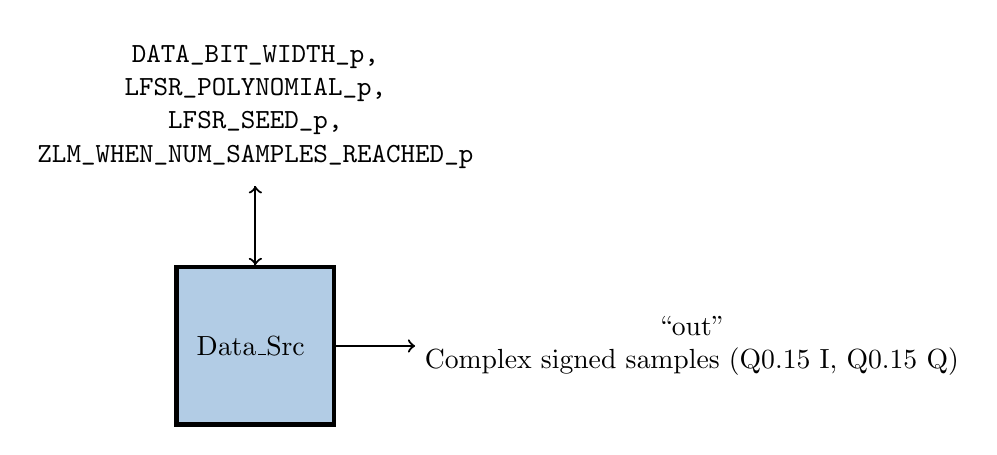
\begin{tikzpicture}[% List of styles applied to all, to override specify on a case-by-case
      every node/.style={
        align=center,     % use this so that the "\\" for line break works
        minimum size=2cm  % creates space above and below text in rectangle
      },
      every edge/.style={draw,thick}
    ]
    \node[rectangle,ultra thick,draw=black,fill=blue](R2){\Comp};
    \node[rectangle,draw=white,fill=white](R4)[right= of R2]{``out'' \\ Complex signed samples (Q0.15 I, Q0.15 Q)};
    \node[rectangle,draw=white,fill=white](R5)[above= of R2]{\verb+DATA_BIT_WIDTH_p,+ \\ \verb+LFSR_POLYNOMIAL_p,+ \\ \verb+LFSR_SEED_p,+ \\ \verb+ZLM_WHEN_NUM_SAMPLES_REACHED_p+};
    \path[->]
    (R2)edge [] node [] {} (R4)
    (R2)edge [] node [] {} (R5)
    (R5)edge [] node [] {} (R2)
    ;
  \end{tikzpicture}
\end{center}\pagebreak

\section*{Source Dependencies}
\subsection*{\comp.hdl}
\begin{itemize}
  \item ocpiassets/components/misc\_comps/data\_src.hdl/data\_src.vhd
  \item ocpiassets/primitives/misc\_prims/lfsr/src/lfsr.vhd
\end{itemize}


\begin{landscape}
	\section*{Component Spec Properties}
	\begin{scriptsize}
% do not delete this line, it is used by the auto gen script to insert latex code
\begin{tabular}{|p{5.5cm}|p{1.25cm}|p{2cm}|p{2.75cm}|p{1.5cm}|p{1.5cm}|p{1cm}|p{5.25cm}|}
\hline
\rowcolor{blue}
Name                 & Type   & SequenceLength & ArrayDimensions & Accessibility       & Valid Range & Default & Usage
\\
\hline
DATA\_BIT\_WIDTH\_p & ushort  & - & - & Parameter & -  &16 & Determines the width of the buses for each of the I and Q data generation memory elements - if less than 16, the most significant \verb+DATA_BIT_WIDTH_p+ bits of I and Q on the out port will be filled. Value is expect to be less than or equal to 16.
\\
\hline
LFSR\_POLYNOMIAL\_p & bool  & - & DATA\_BIT\_WIDTH\_p & Parameter & -  &0 & E.g., a value of 1,1,0,1 would correspond to an LFSR polynomial of \begin{equation*}x^4 + x^3 + (0*x^2) + x^1 + 1\end{equation*} (+1 is always implied regardless of value).
\\
\hline
LFSR\_SEED\_p & bool  & - & DATA\_BIT\_WIDTH\_p & Parameter & -  &0 & Out-of-reset value of the Linear Feedback Shift Register (only affects output data in LFSR mode). This value should never be all zeros, which would cause the register to always have a value of all zeros regardless of polynomial value.
\\
\hline
ZLM\_WHEN\_NUM\_SAMPLES\_REACHED\_p & bool  & - & - & Parameter & -  &false & When value is true and \verb+num_samples+ property value is not -1, worker will generate Zero-Length-Message after \verb+num_samples+ amount of samples have been sent out the output port.
\\
\hline
messageSize\_bytes & ulong  & - & - & Readable, Initial & -  &4096 & Message size in bytes. When the value of (\verb+num_samples+ * num bytes per sample) is less than this property's value, the value of (\verb+num_samples+ * num bytes per sample) is used as the message size.
\\
\hline
num\_samples & long  & - & - & Readable, Writeable & -  &-1 & Maximum number of samples which will be sent out of the output port once out of reset. Note that samples are only sent when the \verb+enable+ property has a value of true. When the value of this property is -1, samples will be sent indefinitely (obeying backpressure from the connected worker, of course).
\\
\hline
fixed\_value & bool  & - & DATA\_BIT\_WIDTH\_p & Readable, Writeable & -  &0x5a5a & The value of this property will be used for I (and the bit-reversed version of this value will be used for Q) to send to the output port when the \verb+mode+ property's value is 'fixed'.
\\
\hline
mode & enum  & - & - & Readable, Writeable & count,walking, LFSR,fixed  &count & Counter, walking ones, Linear Feedback Shift Register, or fixed value.
\\
\hline
enable & bool  & - & - & Readable, Writeable & -  &true & When the worker is not in reset, this property must have a value of true for the data to be sent to the output.
\\
\hline
LFSR\_bit\_reverse & bool  & - & - & Readable, Writeable & -  &true & Used to determine the LFSR shift direction. When true, the \verb+DATA_BIT_WIDTH_p+-bits wide LFSR will be reversed for both I and Q.
\\
\hline
\end{tabular}
%GEN_SPEC_TABLE
	\end{scriptsize}

	\section*{Worker Properties}
	\subsection*{\comp.hdl}
	\begin{scriptsize}
% do not delete this line, it is used by the auto gen script to insert latex code
%GEN_WORKER_TABLE
	\end{scriptsize}

	\section*{Component Ports}
	\begin{scriptsize}
% do not delete this line, it is used by the auto gen script to insert latex code
\begin{tabular}{|M{2cm}|M{1.5cm}|M{4cm}|c|c|M{9cm}|}
\hline
\rowcolor{blue}
Name & Producer & Protocol & Optional & Advanced & Usage
\\
\hline
out & true & iqstream\_protocol& False & ZeroLengthMessages=true & Complex signed samples (Q0.15 I, Q0.15 Q). This port generates data while obeying backpressure. This port is disabled when either the enable property has a value of false or when the \verb+num_samples+ property has a value of greater than 0 and \verb+num_samples+ amount of samples have been sent out this port.\\
\hline
\end{tabular}
%GEN_PORT_TABLE
	\end{scriptsize}

	\section*{Worker Interfaces}
	\subsection*{\comp.hdl}
	\begin{scriptsize}
\begin{tabular}{|M{2cm}|M{1.5cm}|M{4cm}|c|M{12cm}|}
\hline
\rowcolor{blue}
Type & Name & DataWidth & Advanced & Usage
\\
\hline
StreamInterface & out & 32 & - & -\\
\hline
\end{tabular}
%GEN_INTERFACE_TABLE
	\end{scriptsize}
\end{landscape}

\section*{Control Timing and Signals}
\subsection*{\comp.hdl}
\begin{flushleft}
  The FIFO worker uses the clock from the Control Plane and standard Control Plane signals.
\end{flushleft}

\section*{Performance and Resource Utilization}
\subsubsection*{\comp.hdl}
\input{../../\ecomp.hdl/utilization.inc}
%data_src.hdl/target-stratix4/data_src.merge.rpt
\iffalse
+-------------------------------------------------------+
; Partition Merge Resource Usage Summary                ;
+-----------------------------------------------+-------+
; Resource                                      ; Usage ;
+-----------------------------------------------+-------+
; Estimated ALUTs Used                          ; 378   ;
;     -- Combinational ALUTs                    ; 378   ;
;     -- Memory ALUTs                           ; 0     ;
;     -- LUT_REGs                               ; 0     ;
; Dedicated logic registers                     ; 270   ;
;                                               ;       ;
; Estimated ALUTs Unavailable                   ; 5     ;
;     -- Due to unpartnered combinational logic ; 5     ;
;     -- Due to Memory ALUTs                    ; 0     ;
;                                               ;       ;
; Total combinational functions                 ; 378   ;
; Combinational ALUT usage by number of inputs  ;       ;
;     -- 7 input functions                      ; 5     ;
;     -- 6 input functions                      ; 72    ;
;     -- 5 input functions                      ; 102   ;
;     -- 4 input functions                      ; 61    ;
;     -- <=3 input functions                    ; 138   ;
;                                               ;       ;
; Combinational ALUTs by mode                   ;       ;
;     -- normal mode                            ; 297   ;
;     -- extended LUT mode                      ; 5     ;
;     -- arithmetic mode                        ; 76    ;
;     -- shared arithmetic mode                 ; 0     ;
;                                               ;       ;
; Estimated ALUT/register pairs used            ; 470   ;
;                                               ;       ;
; Total registers                               ; 270   ;
;     -- Dedicated logic registers              ; 270   ;
;     -- I/O registers                          ; 0     ;
;     -- LUT_REGs                               ; 0     ;
;                                               ;       ;
;                                               ;       ;
; I/O pins                                      ; 129   ;
; DSP block 18-bit elements                     ; 0     ;
; Maximum fan-out                               ; 270   ;
; Total fan-out                                 ; 2670  ;
; Average fan-out                               ; 2.95  ;
+-----------------------------------------------+-------+
\fi

%data_src.hdl/target-1-stratix4/data_src.merge.rpt
\iffalse
+-------------------------------------------------------+
; Partition Merge Resource Usage Summary                ;
+-----------------------------------------------+-------+
; Resource                                      ; Usage ;
+-----------------------------------------------+-------+
; Estimated ALUTs Used                          ; 377   ;
;     -- Combinational ALUTs                    ; 377   ;
;     -- Memory ALUTs                           ; 0     ;
;     -- LUT_REGs                               ; 0     ;
; Dedicated logic registers                     ; 269   ;
;                                               ;       ;
; Estimated ALUTs Unavailable                   ; 10    ;
;     -- Due to unpartnered combinational logic ; 10    ;
;     -- Due to Memory ALUTs                    ; 0     ;
;                                               ;       ;
; Total combinational functions                 ; 377   ;
; Combinational ALUT usage by number of inputs  ;       ;
;     -- 7 input functions                      ; 7     ;
;     -- 6 input functions                      ; 80    ;
;     -- 5 input functions                      ; 99    ;
;     -- 4 input functions                      ; 46    ;
;     -- <=3 input functions                    ; 145   ;
;                                               ;       ;
; Combinational ALUTs by mode                   ;       ;
;     -- normal mode                            ; 294   ;
;     -- extended LUT mode                      ; 7     ;
;     -- arithmetic mode                        ; 76    ;
;     -- shared arithmetic mode                 ; 0     ;
;                                               ;       ;
; Estimated ALUT/register pairs used            ; 477   ;
;                                               ;       ;
; Total registers                               ; 269   ;
;     -- Dedicated logic registers              ; 269   ;
;     -- I/O registers                          ; 0     ;
;     -- LUT_REGs                               ; 0     ;
;                                               ;       ;
;                                               ;       ;
; I/O pins                                      ; 129   ;
; DSP block 18-bit elements                     ; 0     ;
; Maximum fan-out                               ; 269   ;
; Total fan-out                                 ; 2671  ;
; Average fan-out                               ; 2.95  ;
+-----------------------------------------------+-------+
\fi

%data_src.hdl/target-virtex6/data_src-xst.out
\iffalse
Device utilization summary:
---------------------------

Selected Device : 6vcx75tff484-2


Slice Logic Utilization:
 Number of Slice Registers:             244  out of  93120     0%
 Number of Slice LUTs:                  320  out of  46560     0%
    Number used as Logic:               320  out of  46560     0%

Slice Logic Distribution:
 Number of LUT Flip Flop pairs used:    467
   Number with an unused Flip Flop:     223  out of    467    47%
   Number with an unused LUT:           147  out of    467    31%
   Number of fully used LUT-FF pairs:    97  out of    467    20%
   Number of unique control sets:        19

IO Utilization:
 Number of IOs:                         129
 Number of bonded IOBs:                   0  out of    240     0%
\fi

%data_src.hdl/target-virtex6/data_src-xst.out
\iffalse
Timing Summary:
---------------
Speed Grade: -2

   Minimum period: 3.690ns (Maximum Frequency: 271.021MHz)
   Minimum input arrival time before clock: 1.939ns
   Maximum output required time after clock: 4.353ns
   Maximum combinational path delay: 3.076ns
\fi

%data_src.hdl/target-1-virtex6/data_src-xst.out
\iffalse
Device utilization summary:
---------------------------

Selected Device : 6vcx75tff484-2


Slice Logic Utilization:
 Number of Slice Registers:             243  out of  93120     0%
 Number of Slice LUTs:                  396  out of  46560     0%
    Number used as Logic:               396  out of  46560     0%

Slice Logic Distribution:
 Number of LUT Flip Flop pairs used:    531
   Number with an unused Flip Flop:     288  out of    531    54%
   Number with an unused LUT:           135  out of    531    25%
   Number of fully used LUT-FF pairs:   108  out of    531    20%
   Number of unique control sets:        19

IO Utilization:
 Number of IOs:                         129
 Number of bonded IOBs:                   0  out of    240     0%
\fi

%data_src.hdl/target-1-virtex6/data_src-xst.out
\iffalse
Timing Summary:
---------------
Speed Grade: -2

   Minimum period: 3.557ns (Maximum Frequency: 281.163MHz)
   Minimum input arrival time before clock: 1.939ns
   Maximum output required time after clock: 4.353ns
   Maximum combinational path delay: 3.076ns
\fi

%data_src.hdl/target-zynq/data_src-xst.out
\iffalse
Device utilization summary:
---------------------------

Selected Device : 7z010clg400-3


Slice Logic Utilization:
 Number of Slice Registers:             244  out of  35200     0%
 Number of Slice LUTs:                  320  out of  17600     1%
    Number used as Logic:               320  out of  17600     1%

Slice Logic Distribution:
 Number of LUT Flip Flop pairs used:    467
   Number with an unused Flip Flop:     223  out of    467    47%
   Number with an unused LUT:           147  out of    467    31%
   Number of fully used LUT-FF pairs:    97  out of    467    20%
   Number of unique control sets:        19

IO Utilization:
 Number of IOs:                         129
 Number of bonded IOBs:                   0  out of    100     0%
\fi

%data_src.hdl/target-zynq/data_src-xst.out
\iffalse
Timing Summary:
---------------
Speed Grade: -3

   Minimum period: 2.927ns (Maximum Frequency: 341.647MHz)
   Minimum input arrival time before clock: 1.525ns
   Maximum output required time after clock: 3.460ns
   Maximum combinational path delay: 2.447ns
\fi

%data_src.hdl/target-1-zynq/data_src-xst.out
\iffalse
Device utilization summary:
---------------------------

Selected Device : 7z010clg400-3


Slice Logic Utilization:
 Number of Slice Registers:             243  out of  35200     0%
 Number of Slice LUTs:                  396  out of  17600     2%
    Number used as Logic:               396  out of  17600     2%

Slice Logic Distribution:
 Number of LUT Flip Flop pairs used:    531
   Number with an unused Flip Flop:     288  out of    531    54%
   Number with an unused LUT:           135  out of    531    25%
   Number of fully used LUT-FF pairs:   108  out of    531    20%
   Number of unique control sets:        19

IO Utilization:
 Number of IOs:                         129
 Number of bonded IOBs:                   0  out of    100     0%
\fi

%data_src.hdl/target-1-zynq/data_src-xst.out
\iffalse
Timing Summary:
---------------
Speed Grade: -3

   Minimum period: 2.838ns (Maximum Frequency: 352.324MHz)
   Minimum input arrival time before clock: 1.525ns
   Maximum output required time after clock: 3.460ns
   Maximum combinational path delay: 2.447ns
\fi

\begin{itemize}
  \item \verb+DATA_WIDTH_p=12+
  \item \verb+LFSR_POLYNOMIAL_p=1,1,1,0,0,0,0,0,1,0,0,0+
  \item \verb+LFSR_SEED_p=0,0,0,0,0,0,0,0,0,0,0,0+
  \item \verb+ZLM_WHEN_NUM_SAMPLES_REACHED_p=true+
\end{itemize}
\begin{scriptsize}
  \begin{tabular}{|c|c|c|c|c|c|c|c|}
    \hline
    \rowcolor{blue}
    Device                      & Registers & LUTs & Fmax        & Memory/Special Functions & GCLK & I/O & Design Suite    \\
    \hline
    Stratix4 EP4SGX230K-C2-F40  & 270       & 378  & -           & -                        & 1    & 129 &     Quartus 12.1 SP1\\
    \hline
    Virtex6 XC6VLX240T-1-FF1156 & 244       & 320 & 271 MHz     & -                        & 1    & 129 & ISE 14.7        \\
    \hline
    Zynq XC7Z020-1-CLG484       & 244       & 320 & 341 MHz     & -                        & 1    & 129 & ISE 14.7        \\
    \hline
  \end{tabular}
\end{scriptsize}
\begin{itemize}
  \item \verb+DATA_WIDTH_p=12+
  \item \verb+LFSR_POLYNOMIAL_p=1,1,1,0,0,0,0,0,1,0,0,0+
  \item \verb+LFSR_SEED_p=0,0,0,0,0,0,0,0,0,0,0,0+
  \item \verb+ZLM_WHEN_NUM_SAMPLES_REACHED_p=false+
\end{itemize}
\begin{scriptsize}
  \begin{tabular}{|c|c|c|c|c|c|c|c|}
    \hline
    \rowcolor{blue}
    Device                      & Registers & LUTs & Fmax        & Memory/Special Functions & GCLK & I/O & Design Suite    \\
    \hline
    Stratix4 EP4SGX230K-C2-F40  & 269       & 377  & -           & -                        & 1    & 129 &     Quartus 12.1 SP1\\
    \hline
    Virtex6 XC6VLX240T-1-FF1156 & 243       & 396 & 281 MHz     & -                        & 1    & 129 & ISE 14.7        \\
    \hline
    Zynq XC7Z020-1-CLG484       & 243       & 396 & 352 MHz     & -                        & 1    & 129 & ISE 14.7        \\
    \hline
  \end{tabular}
\end{scriptsize}

\section*{Test and Verification}
\begin{flushleft}
\justify
For verification, multiple test are run with varying values for the \verb+num_samples+ property for each of the available data source modes. The output file is checked for expected length and data contents, with the data content check being specific to the given data source mode.
\end{flushleft}
\end{document}
